\documentclass[conference]{IEEEtran}

\usepackage{cite}
\usepackage{amsmath,amssymb,amsfonts}
\usepackage{algorithmic}
\usepackage{graphicx}
\usepackage{textcomp}
\usepackage{xcolor}
\usepackage{booktabs}
\usepackage{multirow}
\usepackage{makecell}
\usepackage{url}
\usepackage{siunitx}
\usepackage{textcase}
\usepackage[hidelinks]{hyperref}

\sisetup{detect-all, round-mode=places, round-precision=4}

\newcommand{\CICIoT}{\NoCaseChange{CICIoT2023}}

\begin{document}

\title{Device-Aware Threshold Personalization:\\ A Controlled Threshold-Calibration Study for\\ Non-IID Federated IoT Anomaly Detection}

\author{
\IEEEauthorblockN{Salaheddine Naslouby\IEEEauthorrefmark{1},
Amina Aboulmira\IEEEauthorrefmark{4},
Mohamed Lachgar\IEEEauthorrefmark{2},
Hamid Hrimech\IEEEauthorrefmark{3}}
\IEEEauthorblockA{\IEEEauthorrefmark{1}\IEEEauthorrefmark{3}\IEEEauthorrefmark{4}LAMSAD Laboratory, National School of Applied Sciences (ENSA),
Hassan First University, Berrechid, Morocco}
\IEEEauthorblockA{\IEEEauthorrefmark{2}L2IS Laboratory, Higher Normal School (ENS),
University Cadi Ayyad, Marrakech, Morocco}
}

\maketitle

\begin{abstract}
This study isolates threshold calibration scope as the sole experimental variable in a federated IoT anomaly-detection pipeline: a fixed FedAvg autoencoder (E=1, full participation) is trained once per seed, and the same encoder, seeds, and per-client score artifacts are reused across shared (B1), per-client (B2), family-mean (B3), and cluster-mean (B4) threshold policies. The primary comparison is B1 vs.\ B2 on N-BaIoT (K=9 physical devices, q=0.95, five seeds). Because B2 sets each client's threshold at its own benign 95th percentile, FPR equalization is expected by construction under stable calibration/test distributions; the empirical contribution is the held-out magnitude, seed consistency, detection-quality tradeoff, and B4's taxonomy-free approximation. Across the five seeds, B2 reduces CV(FPR) from 1.017 to 0.299 (delta 0.718, bootstrap CI [0.647, 0.769], all five seed deltas positive), and B4 recovers about 52\% without a taxonomy. The gain is not uniform: lower-tail Macro-F1 degradation concentrates in a single low-separability client, and under the randomized file-level CICIoT2023 partition (Regime~B; pseudo-clients, not physical devices), where benign distributions are near-homogeneous, no improvement is observed. These findings are bounded by nine devices, E=1 (which limits local drift), five seeds, and CICIoT2023 conclusions that hold only under the tested partition.
\end{abstract}

\begin{IEEEkeywords}
federated learning, IoT anomaly detection, threshold calibration, false-positive-rate dispersion, autoencoder, non-IID data, personalization.
\end{IEEEkeywords}

\section{Introduction}
\label{sec:introduction}

Federated learning (FL) trains shared models without pooling raw traffic~\cite{mcmahan2017communication}.
Reconstruction-error autoencoders (AEs) are a natural fit for IoT intrusion detection
because benign-only training suffices and attack labels are not required at training time.

A standard deployment trains one shared AE via FedAvg, then applies a threshold $\tau$
above which a reconstruction error signals an intrusion.
In homogeneous fleets this works well.
In heterogeneous fleets, however, benign reconstruction-error distributions differ
substantially across device types: a single shared $\tau$ imposes unequal false-positive
rates (FPRs).
Some devices carry a disproportionate false-alarm burden---making them noisy
or operationally unusable---while others may become under-sensitive.
A shared server-broadcast threshold is natural in deployments where the system
exposes a single global alarm boundary or where per-client threshold state is
not managed independently.

This study asks how large the per-client FPR disparity is under a shared threshold,
how much per-client calibration reduces it, and what detection-quality tradeoff
this creates---all under a fixed FedAvg AE with real physical-device heterogeneity.
The target operational scenario is a fleet of physical IoT devices for which
local benign calibration data are available, and where reducing unequal
false-alarm burden across devices is a deployment priority.
Prior FL-AE work may report aggregate detection metrics or use thresholds implicitly,
but without fixing the encoder, aggregation protocol, and training hyperparameters and
varying only threshold scope, it is impossible to attribute per-client alarm-rate
dispersion to the threshold policy rather than to training differences.
This controlled-comparison gap motivates the present study.

The primary metric is the coefficient of variation of FPR across eligible clients,
$\text{CV(FPR)} = \sigma_{\text{FPR}} / \mu_{\text{FPR}}$.
Four threshold policies are evaluated: a client-averaged shared threshold (B1), full per-client
personalization (B2), device-family grouping (B3), and unsupervised cluster grouping (B4).
B1 is constructed as the arithmetic mean of eligible clients' local 95th-percentile
benign calibration thresholds, broadcast as a single scalar.
The arithmetic mean treats eligible clients equally and models a simple server-broadcast
threshold derived from local calibration summaries, avoiding sample-count domination;
pooled and sample-weighted alternatives are reported as sensitivity checks.
A centralized baseline (B0) is included as a privacy-incompatible reference
comparator but is not part of the single-variable B1--B4 comparison.

The study uses N-BaIoT~\cite{meidan2018n} as the primary confirmatory regime (Regime~A),
CICIoT2023~\cite{neto2023ciciot2023} as a file-level applicability check under
near-homogeneous conditions (Regime~B), and synthetic Dirichlet partitions of N-BaIoT as a
heterogeneity severity sweep (Regime~C).
Five random seeds are used; seed-level descriptive summaries (mean, SD, range, sign consistency) report stability.
The FL simulation uses Flower~\cite{beutel2020flower}.

\textbf{Contributions.}
\begin{itemize}
  \item \emph{Scientific contribution:} A controlled threshold-calibration study
        fixing the FedAvg AE ($E{=}1$, full participation), training protocol, and seeds
        across B1--B4; only the post-training threshold scope varies.
        Because B2 uses each client's own benign $p_{95}$ threshold, FPR equalization
        is expected by construction under stable distributions; the contribution is the
        controlled held-out measurement, seed consistency, tradeoff characterization,
        and B4 approximation---all under a fixed encoder.
  \item \emph{Measured result:} B2 reduces CV(FPR) from $\approx 1.02$ to $0.299$
        (95\% bootstrap CI on $\Delta$: $[0.647,\,0.769]$, all five seed deltas positive;
        relative reduction $(\text{CV}_{\text{B1}} - \text{CV}_{\text{B2}})/\text{CV}_{\text{B1}} = 70.6\%$).
        The detection-quality cost is characterized: P10 Macro-F1 degrades in a single
        low-separability client.
  \item \emph{Scope and limits:} Under the CICIoT2023 randomized file-level pseudo-client
        partition (not physical devices), no improvement is observed.
        A Dirichlet severity sweep is consistent with the benefit concentrating under
        stronger heterogeneity.
  \item \emph{Replication artifact:} Source code, configs, per-seed results, and
        table/figure generation scripts archived on Zenodo
        (DOI: \nolinkurl{10.5281/zenodo.20315654}).
\end{itemize}

\section{Related Work}
\label{sec:related}

\textbf{FL autoencoders for IoT anomaly detection.}
Rey~et~al.~\cite{rey2022federated}, Khraisat~et~al.~\cite{khraisat2025fediot},
and Olanrewaju~et~al.~\cite{olanrewajugeorge2025flae}
apply federated autoencoders to device-partitioned N-BaIoT and report aggregate detection
metrics.
Thresholds are applied implicitly or globally; none isolates threshold calibration scope
as a variable or measures per-client FPR dispersion.

\textbf{Non-IID aggregation.}
Nguyen~et~al.~\cite{nguyen2025fedmse} improve AUC under Dirichlet non-IID N-BaIoT
by weighting aggregation (FedMSE); the approach modifies the training/aggregation protocol,
not the post-training threshold policy, and per-client alarm-rate dispersion is not reported.
General non-IID benchmarks~\cite{zhao2018noniid,li2022federated} focus on loss
and accuracy rather than per-client alarm-boundary dispersion.

\textbf{Model-level FL personalization.}
Personalization in FL is studied mainly at the model level~\cite{fallah2020personalized,arivazhagan2019federated,liang2020think}:
methods such as Per-FedAvg, FedPer, and LG-FedAvg modify model weights or training
objectives to adapt to local distributions.
These approaches adapt the model parameters; DATP instead fixes the shared AE and
adapts only the post-training alarm boundary---the two adaptation layers are complementary.

\textbf{Threshold-level personalization.}
Per-device thresholds are a natural deployment option acknowledged in
Kitsune~\cite{mirsky2018kitsune} and in DIoT~\cite{nguyen2019diot}, but neither provides
a controlled comparison fixing all other variables.
The existence of local thresholds is not new; the missing element is
a controlled study that fixes encoder, training protocol, and seeds across
threshold-scope variants and then measures per-client FPR dispersion.

Table~\ref{tab:related_comparison} summarizes the gap.

\begin{table}[t]
  \caption{Positioning: adaptation layer and threshold treatment.}
  \label{tab:related_comparison}
  \centering
  \resizebox{\columnwidth}{!}{%
  \renewcommand{\arraystretch}{1.2}%
  \begin{tabular}{lll}
    \toprule
    Work group & Adaptation layer & Threshold treatment \\
    \midrule
    FL-AE IoT IDS~\cite{rey2022federated,khraisat2025fediot} & Model (shared AE) & Implicit/global \\
    FedMSE~\cite{nguyen2025fedmse} & Aggregation weights & Not varied \\
    Per-FedAvg, FedPer~\cite{fallah2020personalized,arivazhagan2019federated} & Model weights/objectives & Not addressed \\
    Kitsune, DIoT~\cite{mirsky2018kitsune,nguyen2019diot} & Local AE & Per-device (no controlled study) \\
    \textbf{DATP (this work)} & \textbf{Threshold only} & \textbf{Controlled comparison} \\
    \bottomrule
  \end{tabular}}
\end{table}

\section{Problem Formulation}
\label{sec:formulation}

\subsection{Notation}
Let $\mathcal{K}=\{1,\dots,K\}$ denote the set of FL clients.
Each client $k$ holds local benign traffic data $\mathcal{D}_k^{\text{ben}}$ and may have
attack data $\mathcal{D}_k^{\text{atk}}$.
An autoencoder $h = g \circ f$ maps input $\mathbf{x} \in \mathbb{R}^d$ to a reconstruction
$\hat{\mathbf{x}} = g(f(\mathbf{x}))$, where $f$ is the encoder and $g$ the decoder.
The reconstruction error is the per-sample mean squared error:
\begin{equation}
  e(\mathbf{x}) = \frac{1}{d}\|\mathbf{x} - \hat{\mathbf{x}}\|_2^2,
\end{equation}
where $d$ is the input dimension.

\subsection{Binary Alarm Decision}
Given a threshold $\tau_k$ for client $k$, the alarm decision is:
\begin{equation}
  \text{anomaly}(\mathbf{x}) = \mathbf{1}[e(\mathbf{x}) > \tau_k].
\end{equation}
The FPR for client $k$ is $\rho_k = \Pr[e(\mathbf{x}) > \tau_k \mid \mathbf{x} \sim \mathcal{D}_k^{\text{ben}}]$.

\subsection{Dispersion Metric}
The primary metric is the coefficient of variation of FPR over eligible clients
$\mathcal{K}_{\mathrm{elig}} \subseteq \mathcal{K}$:
\begin{equation}
  \text{CV(FPR)} = \frac{\sigma_{\rho}}{\mu_{\rho}},\quad
  \mu_{\rho} = \frac{1}{|\mathcal{K}_{\mathrm{elig}}|}\sum_{k\in\mathcal{K}_{\mathrm{elig}}} \rho_k,
\end{equation}
where $\sigma_{\rho}$ is the standard deviation.
CV(FPR) normalizes cross-client FPR dispersion by the fleet mean, making dispersion
comparable across regimes with different mean FPR levels; we report IQR(FPR) and
max--min FPR as absolute-dispersion checks to guard against small-denominator artifacts.

\textbf{Eligibility and fallback.}
Eligible clients $\mathcal{K}_{\mathrm{elig}}$ are those with at least $n_{\min}{=}100$ benign calibration samples.
Clients below this threshold are \emph{calibration-pending}: they receive the client-averaged
shared threshold $\tau_{\text{global}}$ (B1 value) as a fallback and are excluded from
dispersion metrics.
Coverage is reported as $|\mathcal{K}_{\mathrm{elig}}|/|\mathcal{K}|$ for all conditions.

\textbf{Operational assumption.}
Percentile calibration assumes each client's benign reconstruction-error distribution
is sufficiently stable between calibration and test.
Temporal drift would weaken the calibration guarantee; this paper does not model concept drift.

\subsection{Confirmatory Statistic}
The primary statistical estimate is the seed-level delta:
\begin{equation}
  \Delta_s = \text{CV(FPR)}_{\text{B1},s} - \text{CV(FPR)}_{\text{B2},s},
\end{equation}
aggregated over seeds $s \in \mathcal{S}$ via descriptive summaries: mean, standard deviation, range, and sign consistency.
With only five seeds, we report these statistics as a seed-level consistency summary---not a high-powered
population significance test.
We interpret all-positive seed deltas as seed-level support
for RQ2 in this tested protocol.

\subsection{Research Questions}
\begin{itemize}
  \item \textbf{RQ1:} Under the client-averaged shared threshold (B1), how large is the variation of FPRs across heterogeneous IoT clients?
  \item \textbf{RQ2:} Does per-client threshold calibration (B2) reduce CV(FPR) compared with the client-averaged shared threshold, and is the reduction consistent across seeds?
  \item \textbf{RQ3:} How much of the B2 dispersion reduction can cluster-mean calibration (B4) recover?
\end{itemize}

The benign calibration-error distributions of different device types differ substantially
in location and spread, so the B1 client-averaged threshold $\tau_{\text{global}}$ crosses
each distribution at a different fraction, producing device-specific FPRs.
Per-client percentile calibration is expected to align benign-tail exceedance rates
when calibration and test distributions are sufficiently stable; the empirical questions
are therefore the magnitude of the FPR-dispersion reduction, the detection-quality
tradeoff it creates, and the extent to which grouped calibration (B4) approximates
per-client calibration without a device taxonomy---all under a fixed FL-AE setting
with real physical-device heterogeneity.

\section{Threshold Personalization Framework}
\label{sec:framework}

Fig.~\ref{fig:per-device-fpr} illustrates the operational consequence of heterogeneous
calibration: under B1 (client-averaged shared~$\tau$), per-device FPRs vary substantially
across the nine N-BaIoT clients, while B2 (per-client~$\tau$) reduces this dispersion for
the representative seed shown.
As an illustrative preview of the primary Regime~A pattern, Fig.~\ref{fig:per-device-fpr}
shows seed~0 only; inference uses the multi-seed results in Table~\ref{tab:regime_a}.

\begin{figure}[t]
  \centering
  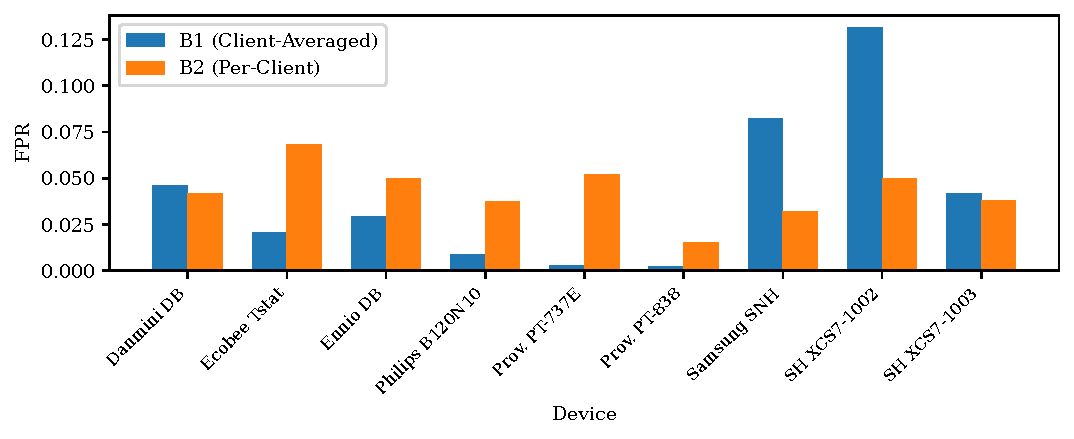
\includegraphics[width=\columnwidth]{figures/figure_1.pdf}
  \caption{Per-device FPR under B1 (Client-Averaged Shared~$\tau$) and B2 (Per-Client~$\tau$)
           for the nine N-BaIoT clients.
           \emph{Illustrative only (seed~0); multi-seed inference uses
           Table~\ref{tab:regime_a} and Table~\ref{tab:per_seed}.}}
  \label{fig:per-device-fpr}
\end{figure}

\begin{figure}[t]
  \centering
  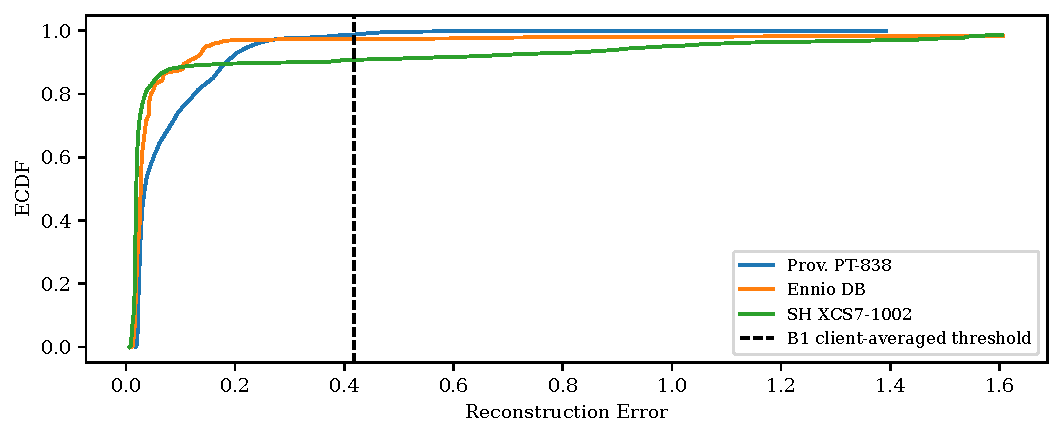
\includegraphics[width=\columnwidth]{figures/figure_2.pdf}
  \caption{Benign reconstruction-error empirical cumulative distributions for three
           representative N-BaIoT clients (seed~0).
           The shared threshold $\tau_{\text{global}}$ (B1, dashed) crosses each curve
           at a different exceedance fraction ($1 - F({\tau})$), producing unequal FPRs.
           Per-client thresholds (B2) set each client's $p_{95}$ independently,
           aligning benign-tail exceedance rates by construction.
           Attack distributions are not shown; they need not shift in parallel with benign tails,
           explaining the TPR/Macro-F1 tradeoff observed in Table~\ref{tab:regime_a}.}
  \label{fig:mechanism}
\end{figure}

\textbf{Pipeline.}
Each client holds benign traffic split into train, calibration, and test partitions;
attack data are reserved exclusively for evaluation and are never used to fit or tune thresholds.
A shared AE is trained with FedAvg via the Flower framework~\cite{beutel2020flower}
(identical training across B1--B4; B0 uses centralized pooling).
\emph{The AE is trained once per (dataset, regime, seed, $\alpha$) condition.}
After training, each client scores its calibration and test data under the fixed AE;
per-client score arrays are written to disk and reused by all threshold policies
without retraining.
Even when a run is budget-capped at 150 rounds, the same final AE state is shared
across all B1--B4 derivations, preserving the threshold-scope-only comparison.

\textbf{Threshold policies.}
Four policies operate on the shared score artifacts:
\begin{itemize}
  \item \textbf{B1 (Client-Averaged):}
        $\tau_{\text{global}} = \frac{1}{|\mathcal{K}_{\mathrm{elig}}|}\sum_{k\in\mathcal{K}_{\mathrm{elig}}} \tau_k^{(95)}$,
        applied uniformly to all clients.
        Pooled and weighted variants are sensitivity checks only
        (Table~\ref{tab:sensitivity_shared}).

  \item \textbf{B2 (Per-Client):} $\tau_k = \tau_k^{(95)}$ applied locally;
        zero additional uplink communication in a deployment where each client
        calibrates its threshold locally.

  \item \textbf{B3 (Family-Mean):} arithmetic mean of local thresholds within each device
        family (Regime~A only; requires a device taxonomy).

  \item \textbf{B4 (Cluster-Mean):} $k$-means on a 4-scalar fingerprint
        $[\mu_e, \sigma_e, \text{skew}_e, p_{95}(e)]$ (StandardScaler-normalized);
        $K{=}3$ for Regime~A, silhouette-selected for Regimes B/C.
        For silhouette selection (Regimes B/C), candidate $K \in \{2,3,4,5\}$;
        $k$-means uses \texttt{k-means++} initialization, $\texttt{n\_init}{=}10$,
        $\texttt{max\_iter}{=}300$, $\texttt{random\_state}{=}42$, applied after
        StandardScaler normalization of the fingerprint matrix.
        Together the four statistics describe the benign calibration-error
        distribution: $\mu_e$ its location, $\sigma_e$ its spread, $\text{skew}_e$
        its tail asymmetry, and $p_{95}(e)$ the operating tail used by thresholding.
        The fingerprint is a grouping input, not a privacy mechanism.
        Regime~A fixes $K{=}3$ because silhouette-based $K$ selection is unstable
        at small $n$ (9 physical devices, coarse device-family structure), and a
        fixed $K$ avoids overfitting the cluster count to sampling noise.
        B4 requires sharing these distributional fingerprints, which carries nonzero
        metadata leakage risk (Section~\ref{sec:threats}).
\end{itemize}

\textbf{Evaluation.}
Each client evaluates FPR, TPR, balanced accuracy, and Macro-F1 on held-out test sets.
CV(FPR), CV(TPR), IQR(FPR), worst-client balanced accuracy, $P_{10}$ Macro-F1 (10th percentile
of per-client Macro-F1 across eligible clients), and coverage ratio are aggregated.
Seed-level deltas are summarized descriptively (mean, SD, range, sign consistency).

\input{sections/experiments}
\section{Results and Discussion}
\label{sec:results}

\subsection{RQ1: FPR Dispersion Under the Client-Averaged Shared Threshold}

Table~\ref{tab:regime_a} presents aggregate results for Regime~A over 5 seeds.
Under B1, CV(FPR) is $1.017 \pm 0.019$---per-client FPRs vary by more than their mean
(a CV above 1 indicates high relative dispersion).
The natural N-BaIoT B1 CV(FPR) ($1.017$) substantially exceeds the IID Dirichlet
baseline ($0.074$), a difference of $0.943$, consistent with device heterogeneity
contributing to the observed dispersion.
B0's CV(FPR) ($0.787$), although lower than B1's, remains substantially above B2 ($0.299$),
consistent with any single pooled or shared scalar threshold crossing heterogeneous
device-error distributions at different exceedance fractions; B0 is included only as a
centralized privacy-incompatible reference, not as part of the controlled B1--B4 ladder.

Fig.~\ref{fig:regime-a-client-fpr} shows per-client FPR distributions.
The worst client (SimpleHome XCS7 security camera) reaches a mean FPR of approximately
$0.122$ while other clients operate near zero, illustrating the unequal alarm-rate
burden imposed by a single shared threshold across heterogeneous devices.

\begin{table}[t]
  \caption{Regime~A (N-BaIoT, $K=9$, coverage~9/9, pending~0): mean $\pm$ std over 5 seeds.
           B0 is a centralized reference, excluded from the B1--B4 controlled ladder.
           Worst BA = worst-client balanced accuracy;
           Mean F1 = mean Macro-F1;
           P10 F1 = 10th-percentile Macro-F1 across eligible clients.}
  \label{tab:regime_a}
  \centering
  \resizebox{\columnwidth}{!}{%
  \renewcommand{\arraystretch}{1.3}%
  \begin{tabular}{lccccccc}
    \toprule
    Baseline & mean FPR & mean TPR & CV(FPR) & CV(TPR) & Worst BA & mean F1 & P10 F1 \\
    \midrule
    B0 (Centralized) & $0.057\pm0.001$ & $0.829\pm0.037$ & $0.787\pm0.031$ & $0.278\pm0.036$ & $0.653\pm0.010$ & $0.720\pm0.054$ & $0.403\pm0.059$ \\
    B1 (Client-Averaged) & $0.039\pm0.002$ & $0.738\pm0.050$ & $\mathbf{1.017\pm0.019}$ & $0.289\pm0.029$ & $0.649\pm0.011$ & $0.563\pm0.068$ & $0.344\pm0.062$ \\
    B2 (Per-Client) & $0.043\pm0.001$ & $0.744\pm0.019$ & $\mathbf{0.299\pm0.073}$ & $0.336\pm0.007$ & $0.651\pm0.001$ & $0.604\pm0.042$ & $0.300\pm0.000$ \\
    B3 (Family-Mean) & $0.051\pm0.006$ & $0.745\pm0.018$ & $0.964\pm0.096$ & $0.336\pm0.007$ & $0.653\pm0.004$ & $0.606\pm0.038$ & $0.299\pm0.000$ \\
    B4 (Cluster-Mean) & $0.044\pm0.003$ & $0.718\pm0.019$ & $0.645\pm0.045$ & $0.322\pm0.012$ & $0.654\pm0.007$ & $0.545\pm0.036$ & $0.299\pm0.000$ \\
    \bottomrule
  \end{tabular}}
  \vspace{2pt}
  {\footnotesize \textbf{Primary result: B1$-$B2 CV(FPR) $\Delta = +0.718$}, SD$\,{=}\,0.079$, seed range $[0.588,\,0.772]$, all 5 deltas positive; B1$-$B4 $\Delta = +0.372$, SD$\,{=}\,0.055$, seed range $[0.319,\,0.443]$.}
\end{table}

\subsection{RQ2: Held-Out FPR-Dispersion Reduction and Detection-Quality Cost}

The primary endpoint is the B1 vs.\ B2 CV(FPR) delta per seed.
Across the five planned seeds, the B1--B2 CV(FPR) deltas are all positive,
with mean $\Delta = 0.718$, SD$\,{=}\,0.079$, and range $[0.588,\, 0.772]$
(Table~\ref{tab:per_seed}).
These seed summaries are reported descriptively rather than as confidence intervals.
A supplementary bootstrap CI (10{,}000 resamples of the five seed-level deltas)
yields $[0.647,\, 0.769]$ at 95\%, excluding zero; given five seeds this is
treated as seed-level consistency evidence under the tested protocol.

Per-client calibration (B2) reduces CV(FPR) from $1.017$ to $0.299$ (coverage: 9/9, pending: 0),
a relative reduction of $70.6\%$,
achieved with zero additional threshold uplink.
B2 requires local threshold state and sufficient benign calibration data;
B4 requires transmitting the 4-scalar fingerprint per client.

The tradeoff with detection uniformity is clear from Table~\ref{tab:regime_a}:
CV(TPR) rises under B2 ($0.336$ vs.\ B1's $0.289$),
worst-client balanced accuracy is comparable (B1: $0.649$, B2: $0.651$),
and mean Macro-F1 improves ($0.604$ vs.\ $0.563$).
However, $P_{10}$ Macro-F1 falls from $0.344$ (B1) to $0.300$ (B2).
B2 slightly increases mean FPR ($0.043$ vs.\ $0.039$) but redistributes
false alarms more evenly; B1 attains a lower fleet-average FPR partly by concentrating
false alarms on high-variance clients.
The near-identical P10 Macro-F1 across B2--B4 ($\approx 0.300$, std $< 0.001$)
reflects a floor effect: the Ennio Doorbell client determines the P10 floor
under B2--B4 in all seeds.
These are distinct failure modes summarized in Table~\ref{tab:failure_modes}.

\begin{table}[t]
  \caption{Client-specific failure modes in Regime~A (5-seed averages).}
  \label{tab:failure_modes}
  \centering
  \footnotesize
  \renewcommand{\arraystretch}{1.2}%
  \begin{tabular}{p{1.4cm}p{1.7cm}p{2.0cm}p{2.2cm}}
    \toprule
    Client & Issue & Evidence & Interpretation \\
    \midrule
    SimpleHome XCS7 & Highest FPR under B1 & Mean FPR $\approx 0.122$ (worst client) & Shared $\tau$ concentrates false alarms on high-variance devices \\
    Ennio Doorbell & P10 Macro-F1 floor under B2--B4 & Lowest AUROC (0.931); 64.9\% attack mass below $p_{95}$ & Benign/attack overlap limits detection after personalization \\
    \bottomrule
  \end{tabular}
\end{table}

Local thresholding controls Ennio's benign false alarms at the cost of
missing the majority of its low-magnitude attack traffic, explaining the P10 Macro-F1
floor.

\textbf{Mechanism.}
Per-client $p_{95}$ thresholding aligns each client's benign tail, mechanically
equalizing false-alarm rates on benign test traffic.
However, attack reconstruction-error distributions need not shift in parallel
with benign distributions: raising the threshold reduces benign false alarms
but can swallow low-magnitude anomaly scores, reducing TPR or lower-tail
Macro-F1 (Fig.~\ref{fig:mechanism} illustrates the benign-side mechanism).
B2 should therefore be interpreted as an FPR-dispersion calibration policy,
not a uniform detection-quality improvement.

All five seed-level deltas are positive (range $0.588$--$0.772$, Table~\ref{tab:per_seed}).

\begin{table}[t]
  \caption{Per-seed CV(FPR) and deltas, Regime~A.
           All $\Delta_{\text{B1-B2}}$ values are positive.
           B4 recovery $= (\text{B1} - \text{B4}) / (\text{B1} - \text{B2})$.}
  \label{tab:per_seed}
  \centering
  \resizebox{\columnwidth}{!}{%
  \renewcommand{\arraystretch}{1.3}%
  \begin{tabular}{cccccc}
    \toprule
    Seed & B1 & B2 & B4 & $\Delta_{\text{B1-B2}}$ & B4 recov.\ (\%) \\
    \midrule
    0 & 1.045 & 0.347 & 0.632 & $+0.698$ & 59.2 \\
    1 & 1.017 & 0.251 & 0.693 & $+0.765$ & 42.3 \\
    2 & 1.015 & 0.243 & 0.654 & $+0.772$ & 46.6 \\
    3 & 1.018 & 0.251 & 0.575 & $+0.767$ & 57.8 \\
    4 & 0.992 & 0.404 & 0.673 & $+0.588$ & 54.3 \\
    \midrule
    Mean & 1.017 & 0.299 & 0.645 & $+0.718$ & 51.8 \\
    \bottomrule
  \end{tabular}}
\end{table}

Absolute FPR dispersion shows the same B1$>$B2 ordering:
IQR(FPR) decreases from $0.035\pm0.002$ (B1) to $0.015\pm0.003$ (B2),
and the max--min FPR gap narrows from $0.120\pm0.007$ to $0.041\pm0.012$.
Because CV(FPR) can be sensitive when mean FPR is small (mean FPR under B1: $0.039$;
under B2: $0.043$), absolute dispersion measures are reported alongside it throughout.
For B1, CV(FPR)$\,{=}\,1.017$ and mean FPR$\,{=}\,0.039$ imply $\sigma_{\text{FPR}} \approx 0.040$;
the CV above~1 therefore reflects genuine cross-client spread comparable to the mean,
not only a small-denominator artifact.

\textbf{Shared-threshold construction sensitivity.}
Pooled and sample-weighted shared-threshold variants preserve the B2 advantage
(Table~\ref{tab:sensitivity_shared}), suggesting the B1-to-B2 reduction is not
driven solely by the arithmetic-mean construction.

\begin{table}[t]
  \caption{Shared-threshold construction sensitivity, Regime~A ($n_{\text{seeds}}=5$, $q=0.95$).
           No AE retraining; sensitivity variants labeled~S.
           All three B1 variants show larger CV(FPR) than B2, consistent with the
           B2 advantage not being driven solely by arithmetic-mean construction.}
  \label{tab:sensitivity_shared}
  \centering
  \resizebox{\columnwidth}{!}{%
  \renewcommand{\arraystretch}{1.3}%
  \begin{tabular}{llcccc}
    \toprule
    Rule & Construction & CV(FPR) & IQR(FPR) & Max--min FPR & $\Delta$ vs B2 \\
    \midrule
    B1 (main) & Arith.\ mean of local $p_{95}$ & $1.017\pm0.019$ & $0.035\pm0.002$ & $0.120\pm0.007$ & $+0.718$ \\
    B1-pooled (S) & Pooled $p_{95}$ & $0.805\pm0.048$ & $0.084\pm0.007$ & $0.134\pm0.012$ & $+0.506$ \\
    B1-weighted (S) & Sample-wt.\ mean of local $p_{95}$ & $0.907\pm0.033$ & $0.050\pm0.018$ & $0.129\pm0.003$ & $+0.608$ \\
    B2 & Per-client $p_{95}$ & $0.299\pm0.073$ & $0.015\pm0.003$ & $0.041\pm0.012$ & --- \\
    \bottomrule
  \end{tabular}}
  {\footnotesize Mean FPR for the main B1/B2 comparison is reported in Table~\ref{tab:regime_a};
   Table~\ref{tab:sensitivity_shared} focuses on dispersion sensitivity across shared-threshold constructions.
   B1-pooled shows lower CV(FPR) than B1 ($0.805$ vs.\ $1.017$) but higher IQR ($0.084$ vs.\ $0.035$):
   because CV normalizes by mean FPR, a pooled threshold that raises mean FPR can reduce
   relative dispersion while absolute spread remains larger.}
\end{table}

\begin{figure}[t]
  \centering
  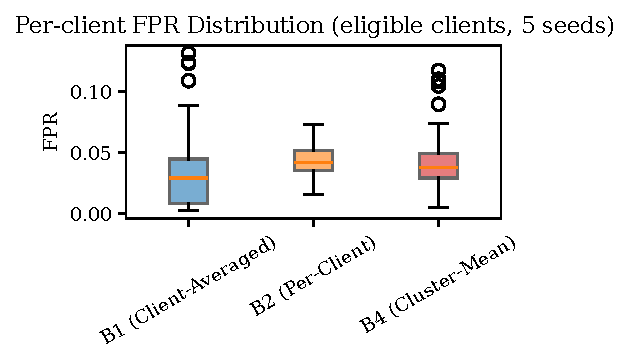
\includegraphics[width=\columnwidth]{figures/figure_3.pdf}
  \caption{Per-client FPR distributions under B1, B2, and B4 (Regime~A, pooled over 5 seeds).
           Descriptive only; inference uses seed-level deltas reported in text.}
  \label{fig:regime-a-client-fpr}
\end{figure}

\subsection{RQ3: Partial Recovery by Cluster-Mean Calibration}

Cluster-mean calibration (B4) achieves CV(FPR) $= 0.645 \pm 0.045$, a partial but consistent improvement over B1.
All five B1$-$B4 deltas are positive (mean $\Delta=0.372$, SD$\,{=}\,0.055$, range $[0.319,\,0.443]$);
all five B4$-$B2 deltas are also positive (mean $\Delta=0.346$, range $[0.269,\,0.442]$).
B4 recovers approximately $52\%$ of B2's improvement (per-seed: $42\%$--$59\%$, Table~\ref{tab:per_seed}).
B4 requires no device taxonomy and transmits only compact 4-scalar fingerprints per client;
however, it does not provide privacy (see Section~\ref{sec:framework}).
Cluster assignments show moderate stability across seeds in Regime~A
(pairwise adjusted Rand index: mean~$0.79$, range $[0.64,\,1.0]$ over all seed pairs).
A post-hoc silhouette check over $K \in \{2,3,4,5\}$ yields mean scores of
$0.29$, $0.31$, $0.34$, and $0.32$ respectively---all low and within $\pm 0.05$---confirming
that the nine-device Regime~A fingerprint space has no clearly dominant cluster count;
$K{=}3$ is a pragmatic fixed choice rather than a structurally optimal partition.
With only nine physical devices, B4 is exploratory and requires validation on larger fleets.
B4's fingerprint still depends on calibration-error statistics including $p_{95}$, so
clients below the eligibility threshold remain calibration-pending and use
$\tau_{\text{global}}$.

Family-mean calibration (B3, Regime~A only) reduces CV(FPR) negligibly
($0.964$ vs.\ B1's $1.017$): the coarse N-BaIoT device-family taxonomy
(Danmini/Ennio doorbells, Ecobee thermostat, Philips baby monitor, Samsung webcam,
Provision/SimpleHome security cameras) does not align with the reconstruction-error
calibration structure---devices within the same family can have dissimilar
benign-error distributions, while devices across families can be similar.
This taxonomy-independence of calibration structure motivates B4's data-driven clustering
over B3's label-based grouping.

\subsection{Regime B: File-Level Applicability Check (CICIoT2023)}

Table~\ref{tab:regime_b} shows Regime~B results.
Under the file-level CICIoT2023 partition, benign reconstruction-error distributions are
near-homogeneous (pairwise JS divergence: mean $0.004$, median $0.003$, max $0.038$
over all $\binom{63}{2}$ pairs and 5 seeds).
B1 achieves CV(FPR) $= 0.099 \pm 0.002$; B2 increases it to $0.133 \pm 0.007$
(all five seed-level B1$-$B2 deltas are negative; mean $-0.034$, SD $0.006$, range $[-0.043,\,-0.026]$).
When benign distributions are near-homogeneous under this file-level partition, the shared
threshold is already a good fit and per-client calibration introduces variance without
benefit---no personalization improvement was observed in this setting.

\textbf{Interpretation caveat.}
Regime~B uses file-defined CICIoT2023 pseudo-clients (not physical devices) with randomized ordering; it is interpreted only as a near-homogeneous applicability boundary.
All runs were budget-capped at 150 rounds; comparisons remain controlled because all policies share the same frozen AE per seed.

\begin{table}[t]
  \caption{Regime~B (\CICIoT{} file-defined clients, $K=63$, coverage~63/63, pending~0): mean $\pm$ std over
           5 seeds, eligible clients only. B3 not applicable. All runs budget-capped at 150 rounds.}
  \label{tab:regime_b}
  \centering
  \resizebox{\columnwidth}{!}{%
  \renewcommand{\arraystretch}{1.3}%
  \begin{tabular}{lcccccc}
    \toprule
    Baseline & mean FPR & mean TPR & CV(FPR) & CV(TPR) & Worst BA & mean Macro-F1 \\
    \midrule
    B0 (Centralized) & $0.051\pm0.001$ & $0.981\pm0.000$ & $0.109\pm0.020$ & $0.001\pm0.000$ & $0.954\pm0.006$ & $0.959\pm0.000$ \\
    B1 (Client-Averaged) & $0.051\pm0.001$ & $0.982\pm0.000$ & $0.099\pm0.002$ & $0.001\pm0.000$ & $0.959\pm0.002$ & $0.959\pm0.000$ \\
    B2 (Per-Client) & $0.051\pm0.001$ & $0.982\pm0.000$ & $0.133\pm0.007$ & $0.001\pm0.000$ & $0.956\pm0.001$ & $0.959\pm0.000$ \\
    B4 (Cluster-Mean) & $0.051\pm0.001$ & $0.982\pm0.000$ & $0.101\pm0.003$ & $0.001\pm0.000$ & $0.959\pm0.002$ & $0.959\pm0.000$ \\
    \bottomrule
  \end{tabular}}
\end{table}

\subsection{Regime C: Non-IID Severity Sweep}

Fig.~\ref{fig:severity} and Table~\ref{tab:regime_c} show that the personalization benefit is broadly consistent with larger gains under stronger
heterogeneity, concentrated in the low-$\alpha$ band and absent under near-IID conditions.
The $\alpha=0.1$ and $\alpha=0.3$ seed ranges overlap ($[0.535,\,0.786]$ vs.\ $[0.420,\,0.897]$),
so strict monotonicity between these two levels should not be inferred from this data;
they form a high-heterogeneity band rather than a strictly ordered pair.
B4 follows the same qualitative pattern but remains a partial approximation.

\begin{figure}[t]
  \centering
  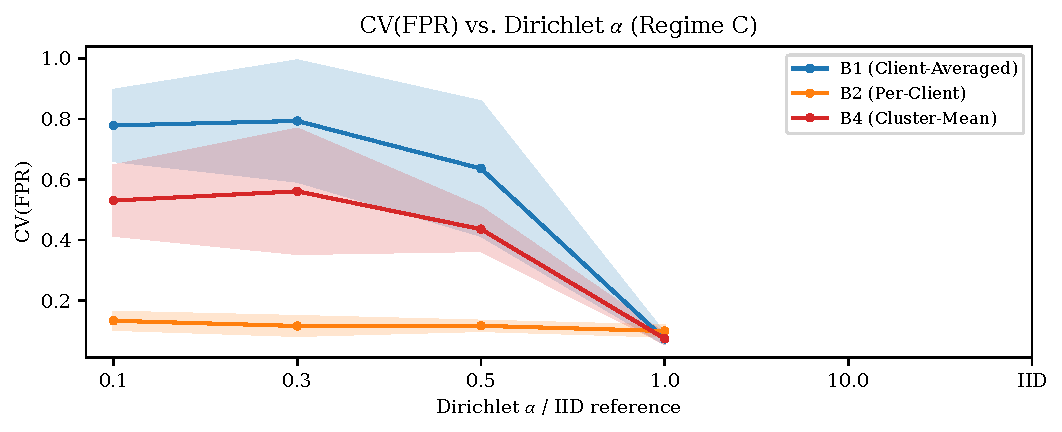
\includegraphics[width=\columnwidth]{figures/figure_4.pdf}
  \caption{Regime C: mean CV(FPR) by threshold strategy as a function of Dirichlet~$\alpha$.
           Whiskers show $\pm$1 std over 5 seeds.
           The B1--B2 gap is largest in the low-$\alpha$ band
           and disappears under IID or near-homogeneous conditions.}
  \label{fig:severity}
\end{figure}

\begin{table}[t]
  \caption{Regime C (N-BaIoT Dirichlet partition, $K=20$):
           mean CV(FPR) $\pm$ std over 5 seeds.
           Mean FPR is $\approx 0.050$ for all $\alpha$ levels and baselines;
           coverage is 20/20 (pending~0) except $\alpha{=}0.1$ where
           coverage is 19--20/20 (pending~0--1).}
  \label{tab:regime_c}
  \centering
  \resizebox{\columnwidth}{!}{%
  \footnotesize
  \setlength{\tabcolsep}{3pt}%
  \renewcommand{\arraystretch}{1.3}%
  \begin{tabular}{lccccc}
    \toprule
    $\alpha$ & B1 CV & B2 CV & B4 CV & $\Delta$ & Seed range \\
    \midrule
    0.1  & $0.779\pm0.104$ & $0.134\pm0.025$ & $0.531\pm0.103$ & $0.645$ & $[0.535,\,0.786]$ \\
    0.3  & $0.793\pm0.178$ & $0.117\pm0.028$ & $0.561\pm0.184$ & $0.677$ & $[0.420,\,0.897]$ \\
    0.5  & $0.636\pm0.197$ & $0.117\pm0.014$ & $0.436\pm0.063$ & $0.519$ & $[0.240,\,0.777]$ \\
    1.0  & $0.544\pm0.116$ & $0.096\pm0.021$ & $0.426\pm0.066$ & $0.448$ & $[0.238,\,0.565]$ \\
    10.0 & $0.174\pm0.053$ & $0.111\pm0.016$ & $0.133\pm0.012$ & $0.063$ & $[0.006,\,0.122]$ \\
    IID  & $0.074\pm0.014$ & $0.100\pm0.015$ & $0.075\pm0.013$ & $-0.026$ & $[-0.032,\,-0.019]$ \\
    \bottomrule
  \end{tabular}}
  \vspace{3pt}
  {\footnotesize $\Delta$\,=\,B1$-$B2 mean delta. Seed range\,=\,descriptive min--max over five seeds, not a confidence interval.}
  \vspace{3pt}
\end{table}

\section{Threats to Validity}
\label{sec:threats}

\textbf{FPR--TPR tradeoff.}
B2 reduces CV(FPR) but increases CV(TPR) ($0.336$ vs.\ $0.289$) and decreases P10 Macro-F1
($0.300$ vs.\ $0.344$); worst-client balanced accuracy is not materially degraded.
Per-client threshold personalization improves false-alarm dispersion fairness, not universal detection quality.

\textbf{Dataset scope.}
Regime A uses 9 physical IoT devices; CV(FPR) is computed over 9 eligible
clients per seed, and bootstrap intervals are computed over the five seed-level deltas.
The core Regime~A evidence is limited to these nine devices, so the paper
does not claim population-level generality over all IoT fleets.
The value of Regime~A is that it uses real physical device identities and
natural device-level benign heterogeneity, making it the correct confirmatory
condition for the paper's mechanism.
Regime~C ($K{=}20$ synthetic clients) helps test whether the effect behaves
consistently as heterogeneity severity changes but is not a replacement for
more physical devices.
Regime~B adds a contrasting near-homogeneous condition showing that the benefit
is conditional, not universal.
The results should therefore be read as a controlled measurement study of
threshold-scope effects under a fixed federated encoder, rather than as
fleet-scale deployment validation.
Future work should test larger multi-vendor physical fleets.

\textbf{CICIoT2023 partition.}
The Regime~B result depends on our file-level CICIoT2023 partition, which produces
near-homogeneous clients.
A different partition (e.g., by attacker type) might yield different client heterogeneity.

\textbf{Calibration data sufficiency.}
In all reported conditions, calibration-pending count is zero.
In deployments with fewer than $n_{\min}=100$ benign calibration samples per client,
B2 and B4 fall back to $\tau_{\text{global}}$, reducing their advantage.

\textbf{Threshold quantile sensitivity.}
$q$ is fixed at $0.95$. A threshold-only sensitivity check over $q \in \{0.90, 0.95, 0.99\}$
preserves the qualitative B2 $<$ B4 $<$ B1 ordering; absolute CV(FPR) values shift with $q$.
The B1-pooled and B1-weighted shared-threshold sensitivity checks are consistent with
the B1-to-B2 gap not being driven solely by the arithmetic-mean construction (Table~\ref{tab:sensitivity_shared}).

\textbf{Attack scope and adversarial robustness.}
The evaluation uses Mirai and BASHLITE variants on N-BaIoT.
No poisoning, backdoor, or evasion evaluation is performed.

\textbf{Privacy.}
Threshold personalization reduces data exposure at calibration but provides no formal differential-privacy or
cryptographic guarantees.
B4 transmits a compact 4-scalar fingerprint $[\mu_e, \sigma_e, \text{skew}_e, p_{95}(e)]$;
this vector can reveal coarse information about the shape, stability, and tail behavior
of a client's benign reconstruction-error distribution.
Concretely, a highly skewed or high-variance fingerprint can reveal irregular or bursty
benign behavior, heavy usage periods, or coarse device behavior class; this is
distributional metadata leakage, not raw traffic leakage and not proof of a
reconstruction attack, but it is not negligible.
Such metadata could help an adversary prioritize devices or time probing attempts
during periods inferred to be high-variance, although this paper does not demonstrate
such an attack.
B4 is not a privacy mechanism.
Mitigations such as secure aggregation, differential privacy, or local-only clustering
are complementary future work, not claims of this paper.

\textbf{Convergence and budget-capped runs.}
Budget-capped runs limit broad convergence interpretation, but within each seed the
same frozen AE is used across B1--B4, preserving threshold-calibration-only attribution.

\textbf{Architecture and aggregation.}
The study uses a fixed AE $[d, 80, 40, 20]$ with vanilla FedAvg ($E{=}1$).
Larger $E$ or different architectures may alter reconstruction-error geometry and the
personalization benefit magnitude; this is future work.

\textbf{Concept drift.}
Local percentile thresholds can become stale when benign device behavior changes over
time, for example after firmware updates, workload changes, or network-policy changes.
This study evaluates fixed train/calibration/test splits and does not model online
recalibration or drift detection; DATP therefore assumes that benign
reconstruction-error distributions remain sufficiently stable between calibration
and deployment.

\textbf{Seeds and statistical power.}
Five seeds provide limited bootstrap power.
CI widths are satisfactory for a positive primary claim but the study is underpowered
for small effect sizes.
All claims are scoped to the tested datasets, partitions, and protocol.

\section{Conclusion}
\label{sec:conclusion}

This study holds the FedAvg AE ($E{=}1$, full participation), training protocol, and seeds fixed across B1--B4;
only the post-training threshold calibration scope varies.
On heterogeneous N-BaIoT devices, per-client calibration (B2) provides the strongest
FPR-dispersion reduction ($\Delta = 0.718$, all five seed deltas positive, range $[0.588,\,0.772]$);
cluster-mean calibration (B4) recovers a meaningful but partial share
($\approx$52\% of B2's improvement) without requiring a device taxonomy, at the cost
of transmitting distributional metadata that is not private.
Family-mean calibration (B3) performs poorly: coarse device-type labels do not align
with reconstruction-error calibration structure.

When benign error distributions are near-homogeneous (CICIoT2023 under the file-level
pseudo-client partition, Dirichlet near-IID), no dispersion reduction is observed---this is
an applicability boundary rather than evidence that personalization is unnecessary for these datasets generally.
The main tradeoff under heterogeneous conditions is that B2 reduces FPR dispersion
and improves mean Macro-F1, but the lower-tail P10 Macro-F1 degradation is concentrated
in the low-separability Ennio Doorbell client---a client-specific failure of percentile
calibration rather than evidence of a universal FPR--TPR tradeoff.
Per-client calibration is an FPR-equity intervention, not a uniform detection-quality improvement.

\textbf{Practitioner guidance.}
First, measure benign calibration-error heterogeneity across clients, for example
using pairwise distribution divergence or dispersion of local calibration thresholds.
Second, choose the threshold policy according to that heterogeneity and deployment
constraints: use B1 when clients are near-homogeneous or per-client state is
undesirable; use B2 when local calibration is available and false-alarm equity is the
priority; use B4 when taxonomy-free grouping is acceptable, while accounting for the
metadata leakage introduced by shared distributional fingerprints.

\textbf{Limitations.}
Regime~A uses only 9 physical devices (B4 is exploratory at this scale);
Regime~B uses randomized file-level pseudo-clients (not physical devices);
$E{=}1$ with full participation limits local drift---results characterize threshold personalization under a frequently synchronized encoder, not drift-heavy settings;
five seeds limit statistical power; no adversarial robustness, formal privacy, or hardware evaluation is provided.
Evaluating $E > 1$ and alternative CICIoT2023 partitions (physical-device, attack-source) is future work.
Threshold personalization is complementary to---not a replacement for---model-level personalization.

\textbf{Future work:} larger physical fleets, $E > 1$ sensitivity,
privacy-preserving grouping, model-level personalization, adversarial robustness,
and deployment validation under concept drift.

\noindent\textbf{Availability.}
A replication package containing source code, configuration files, per-seed results,
and table/figure generation scripts is archived on Zenodo (DOI: 10.5281/zenodo.20315654).
Detailed reproduction commands are provided in the repository documentation.


\bibliographystyle{IEEEtran}
\bibliography{references}

\end{document}
